\documentclass[a4paper]{article}
\usepackage[14pt]{extsizes} 
\usepackage[T2A]{fontenc}
\usepackage[utf8]{inputenc}
\usepackage{natbib}
\usepackage{graphicx}
\usepackage{amsmath}
\usepackage[english]{babel}
\usepackage{fontspec}
\usepackage{amsmath,amsfonts,amssymb,amsthm,mathtools,mathrsfs}
\usepackage{icomma}
\usepackage{fullpage}
\usepackage{ulem}
\usepackage{eufrak}
\usepackage{setspace}
\usepackage{listings}
\usepackage{indentfirst}
\usepackage[left=2cm,right=1.5cm,top=2cm,bottom=2cm]{geometry}
\usepackage{xcolor}
\usepackage{float}
\usepackage{csquotes}

\setmainfont[Ligatures={TeX,Historic}]{Times New Roman}
\setlength{\parindent}{5ex}
\setlength{\parskip}{1em}
\renewcommand{\baselinestretch}{1}

\graphicspath{{images/}}

\definecolor{buzzlightyear}{HTML}{8757A5}
\definecolor{grass}{HTML}{738D06}
\definecolor{literal}{HTML}{F18A2B}
\definecolor{commentcolor}{HTML}{8E908B}

\lstdefinestyle{habrstyle}{
    backgroundcolor=\color{white},   
    commentstyle=\color{commentcolor},
    keywordstyle=\bfseries\color{buzzlightyear},
    numberstyle=\tiny\color{commentcolor},
    stringstyle=\color{grass},
    basicstyle=\ttfamily\footnotesize,
    breakatwhitespace=false,         
    breaklines=true,                 
    captionpos=b,                    
    keepspaces=true,                 
    numbers=left,                    
    numbersep=5pt,                  
    showspaces=false,                
    showstringspaces=false,
    showtabs=false,                  
    tabsize=4
}

\lstset{style=habrstyle}

\begin{document}

    % FIRST PAGE
    \begin{center}
        \begin{center}
        \hfill \break
        \normalsize{Санкт-Петербургский государственный политехнический}\\
        \normalsize{университет Петра Великого}\\
        \hfill \break
        \normalsize{\textbf{Высшая школа интеллектуальных систем и}}\\ 
        \normalsize{\textbf{суперкомпьютерных технологий}}\\ 
        \hfill \break
        \hfill \break
        \hfill \break
        \normalsize{Лабораторная работа}\\
        \hfill \break
        \hfill \break
        \normalsize{\LARGE Автокорреляция}\\
        \end{center}
        \hfill \break
        \hfill \break
        \hfill \break
        \hfill \break
        \hfill \break
        \hfill \break
        \hfill \break
        \hfill \break
        \hfill \break
        \hfill \break
        \begin{flushright}
            \normalsize{Работу выполнил студент}\\
            \normalsize{3-го курса, группа 3530901/80201}\\
            \normalsize{Сахибгареев Рамис Ринатович}\\
            \hfill \break
            \normalsize{Преподаватель:}\\
            \normalsize{Богач Наталья Владимировна}\\
        \end{flushright}
        \hfill \break
        \hfill \break
        \hfill \break
        \hfill \break
        \begin{center} Санкт-Петербург 2021 \end{center}
        \thispagestyle{empty}
    \end{center}
    % FIRST PAGE [END]
    
    \newpage
        \tableofcontents
    
    \newpage
         \listoffigures
    
    \newpage
         \lstlistoflistings   
     
    % START START START START START
    \newpage
        \section{Part 1: Vocal chirp's pitch estimation}
        
        We cannot define pitch of the signal at the moment, because of low frequency resolution. Also we cannot increase window size because signal is non-periodic. But we can use auto-correlation. Let's write some functions, that allows us to find windows correlation.
        
        \begin{lstlisting}[language=Python,caption=sserial-corr and autocorr functions,label={lst:part1_1}]
    from thinkdsp import *
    import thinkplot
    
    def serial_corr(wave, lag=1):
        N = len(wave)
        y1 = wave.ys[lag:]
        y2 = wave.ys[:N-lag]
        corr = np.corrcoef(y1, y2)[0, 1]
        return corr
    def autocorr(wave):
        lags = np.arange(len(wave.ys)//2)
        corrs = [serial_corr(wave, lag) for lag in lags]
        return lags, corrs
        \end{lstlisting}
        
        After defining these functions we can apply them to the vocal signal.
        
        \begin{lstlisting}[language=Python,caption=Vocal signal lag correlation estimation,label={lst:part1_1}]
    wave = read_wave('data/voice.wav')
    segment = wave.segment(start=0, duration=0.01)
    lags, corrs = autocorr(segment)
    lag = np.array(corrs[90:110]).argmax() + 90
    thinkplot.plot(lags, corrs , color = 'blue')
    thinkplot.config(xlabel='Lag', ylabel='Correlation')
    print(segment.framerate / lag)
        \end{lstlisting}
        
        \begin{figure}[H]
            \centering
            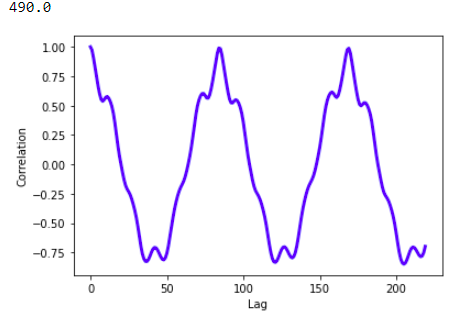
\includegraphics[width=\textwidth]{img/corr_lag.png}
            \caption{Vocal signal lag correlation}
            \label{fig:part1_1_1}
        \end{figure}
        
    \newpage
        \section{Part 2: Signal pitch plot calculation}

        To automate process of the previous part, let's write a little function, that returns estimated frequency.
        
        \begin{lstlisting}[language=Python,caption=Log spectrum,label={lst:part1_2}]
    def estimate_fundamental(segment , low=70, high=150):
        lags, corrs = autocorr(segment)
        lag = np.array(corrs[low:high]).argmax() + low
        period = lag / segment.framerate
        frequency = 1 / period
        return frequency
        \end{lstlisting}
        
        Now let's build the signal's spectrogram. We can clearly see a main spike.
        
        \begin{lstlisting}[language=Python,caption=Segment frequency estimator,label={lst:part1_2}]
    def estimate_fundamental(segment , low=70, high=150):
        lags, corrs = autocorr(segment)
        lag = np.array(corrs[low:high]).argmax() + low
        period = lag / segment.framerate
        frequency = 1 / period
        return frequency
        \end{lstlisting}
        
        \begin{figure}[H]
            \centering
            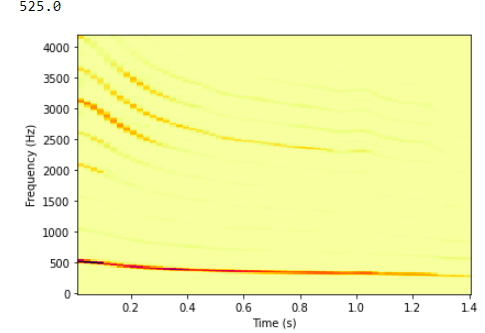
\includegraphics[width=\textwidth]{img/voice_spec.png}
            \caption{Voice signal spectrogram}
            \label{fig:part1_1_2}
        \end{figure}
        
        We can estimate accuracy of our function by splitting the signal into the small parts and estimating the frequency of each part. After we can apply this values to the plot and check, how estimated frequency close to the real.
            
        \begin{lstlisting}[language=Python,caption={Estimation check code},label={lst:sawtooth_def}]
    starts = np.arange(0.0, 1.4, 0.05)
    ts = []
    freqs = []
    for start in starts:
        ts.append(start + 0.05/2)
        segment = wave.segment(start=start , duration=0.01)
        freq = estimate_fundamental(segment)
        freqs.append(freq)
    wave.make_spectrogram(2048).plot(high=1000)
    plt.plot(ts, freqs , color='aqua', linewidth=4)
    decorate(xlabel='Time (s)', ylabel='Frequency (Hz)')
        \end{lstlisting}
        
        \begin{figure}[H]
            \centering
            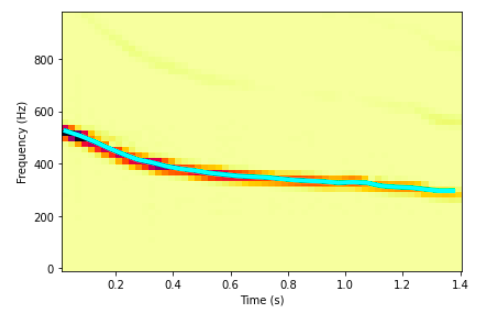
\includegraphics[width=\textwidth]{img/voice_freq.png}
            \caption{Voice signal spectrogram and estimated frequency}
            \label{fig:part1_1_2}
        \end{figure}
        
        We can clearly see, that estimated frequency follows main spectrogram spike.
        
    \newpage
        \section{Part 3: GREATEST CRYPTOCURRENCY OF ALL TIME (aka. bitcoin). PART 2}
            
        In this part we need to try to apply autocorrelation method to the bitcoin chart. 
        
        Code for parsing the .csv file is the same, as it was in the previous lab.
        
        \begin{lstlisting}[language=Python,caption=Bitcoin to a wave,label={lst:als_sqr}]
    data = pd.read_csv('data/bitcoin.csv')
    price = data['Closing Price (USD)']
    count = data.index
    wave = Wave(price,count,framerate=1)
    wave.plot()
    decorate(xlabel='Day')
        \end{lstlisting}
            
        \begin{figure}[H]
            \centering
            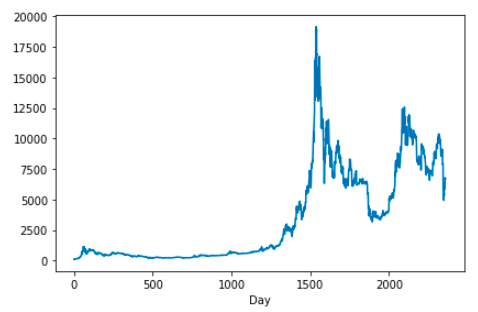
\includegraphics[width=\textwidth]{img/btc.png}
            \caption{Bitcoin chart}
            \label{fig:als_sqr}
        \end{figure}
        
        Let's look, how looks a logarithmic graph of a spectrum's power.
        
        \begin{lstlisting}[language=Python,caption=Bitcoin autocorrelation estimation,label={lst:als_sqr}]
    lags, corrs = autocorr(wave)
    thinkplot.plot(lags, corrs)
    decorate(xlabel='Lag', ylabel='Correlation')
        \end{lstlisting}
        
        \begin{figure}[H]
            \centering
            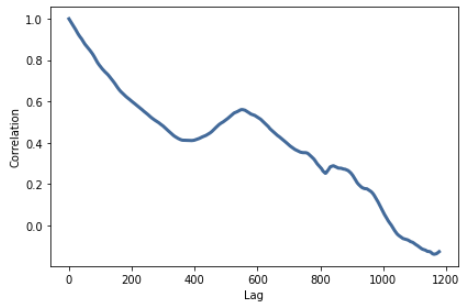
\includegraphics[width=\textwidth]{img/btc_corr.png}
            \caption{Bitcoin's autocorrelation}
            \label{fig:als_clr}
        \end{figure}
            
        As we can see, bitcoin has no signs of a periodic signal, so we cannot predict its values.
            
    \newpage
        \section{Part 4: Missing fundamental}
        
            In this part we need to explore Missing Fundamental effect.
            
            To do it we can use existing notebook, that uses saxophone record to demonstrate this effect.
            
            Firstly, let's take a look on the record spectrogram.
            
            \begin{figure}[H]
                \centering
                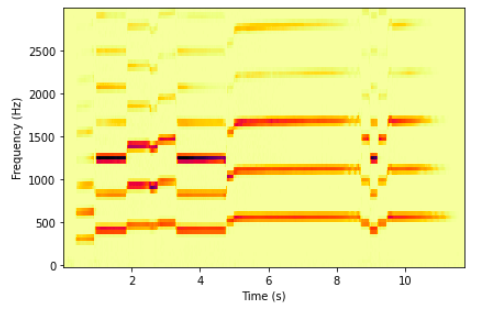
\includegraphics[width=\textwidth]{img/sac_spectr.png}
                \caption{Saxophone record spectrogram}
                \label{fig:part42}
            \end{figure}
            
            We can clearly see spikes, spectrum of the stable segment also confirms it.
            
            \begin{figure}[H]
                \centering
                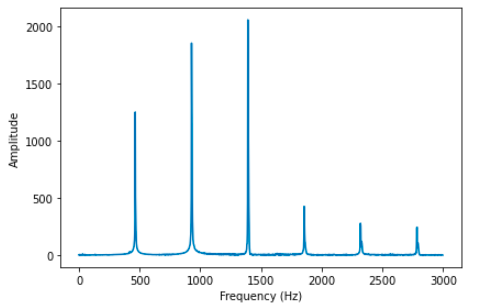
\includegraphics[width=\textwidth]{img/sac_spec.png}
                \caption{Saxophone record spectrum}
                \label{fig:part42}
            \end{figure}
            
            Triangle signal with same fundamental frequency hears differently - with more lower pitch.
            Let's take a look on the correlation plot.
            
            \begin{figure}[H]
                \centering
                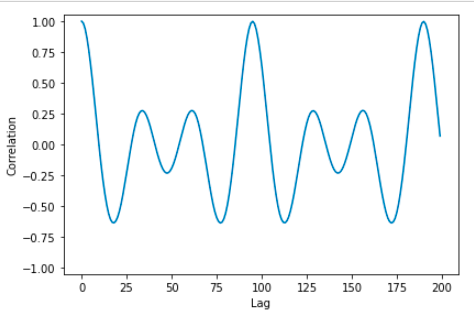
\includegraphics[width=\textwidth]{img/sac_corr.png}
                \caption{Saxophone correlation}
                \label{fig:part42}
            \end{figure}
            
            We can clearly see spike on the frequency of 464 Hz.
            But what would happen, if we cutoff this frequency from the signal? Let's check out.
            
            \begin{figure}[H]
                \centering
                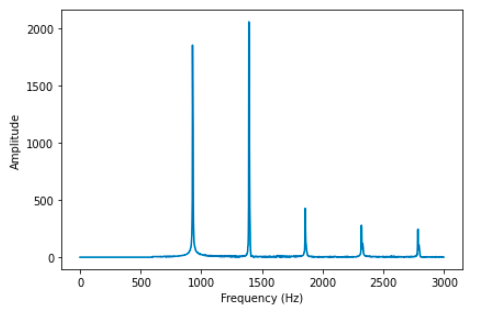
\includegraphics[width=\textwidth]{img/sac_filt.png}
                \caption{Saxophone spectrum without 464 Hz harmonic}
                \label{fig:part42}
            \end{figure}
            
            However, If we listen new record, we won't find pitch difference.
            Also if we take a look on the correlation plot, we won't find any difference too.
            
            \begin{figure}[H]
                \centering
                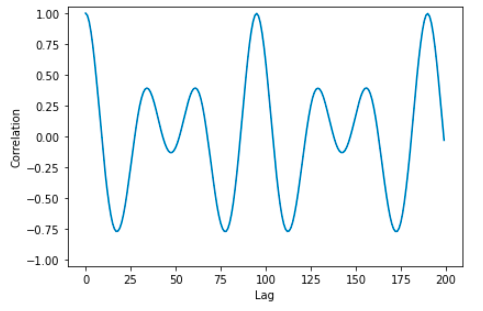
\includegraphics[width=\textwidth]{img/sac_corr_2.png}
                \caption{Saxophone correlation plot filtered}
                \label{fig:part42}
            \end{figure}
            
            This effect called missing fundamental - even when we removed fundamental harmonic it remains fundamental frequency of the signal. But if we remove its high frequency factors from the signal too, then no traces of the original signal would left.
            
            \begin{figure}[H]
                \centering
                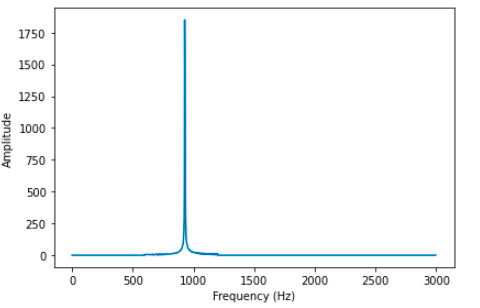
\includegraphics[width=\textwidth]{img/sac_filtered_hard.png}
                \caption{Saxophone spectrum plot filtered hard}
                \label{fig:part42}
            \end{figure}
            
            \begin{figure}[H]
                \centering
                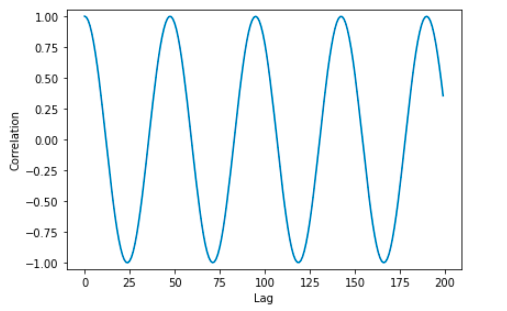
\includegraphics[width=\textwidth]{img/sac_corr_3.png}
                \caption{Saxophone correlation plot filtered hard}
                \label{fig:part42}
            \end{figure}
    
    \newpage
        \section{Conclusion}
            We've learned, what autocorrelation is, how we can compute it and how it affects the signals. Autocorrelation can be used to estimate fundamental frequency of the signal or say, that signal is chaotic and there is no period. Autocorrelation is a reason of missing fundamental effect, when out ears can hear phantom base frequency even if signal doesn't have a harmonic with this frequency.
     
\end{document}
